%\documentclass[aspectratio=169]{beamer}
\documentclass{beamer}
\usepackage[utf8x]{inputenc}
%\usepackage{default}
\usepackage{verbatim}
\usepackage{graphicx}
\usepackage{transparent}
\usepackage{listings}
\usepackage{qtree}
\usepackage{amsmath}

% Table of contents weg (DONE)
% slides nummeren (DONE)
% introslide over ons algehele probleem al een plaatje laten zien van de boeken (DONE)
% conclusie data set bekijken: challenges: verschil kwaliteit (in teksts neerzetten) (DONE)

% Introslide laten zien (met onze 2 stappen, sfm en crfs ssvm), overview methode + annotater tool
%   als 0de stap toevoegen
% page classification en image localization tegelijk laten zien (weer met plaatjes)
% HOG features uitleggen (algemeen HOG feature plaatje, uitleggen hoe je dit
%   plaatje moet laten lezen)
% voorbeeldslides HOG features

% vraag: wat voor schaal voor de HOG hebben we gebruikt (grootte filter)
% HOGgles runnen om te kijken waarom ons project zo faalt

% discussion: focus ook op goede dingen






\DeclareMathOperator*{\argmin}{arg\,min}

\title{Plucking Pictures from Publications}
\subtitle{I don't know what I'm doing!}
\author{Maarten Inja \and Maarten de Waard}
\institute[UvA]{University of Amsterdam}
\date[2014]{Intelligent Systems Project, June 26, 2014}
\logo{
\includegraphics[width=45px]{resources/uva}}
\usetheme{Berkeley}
\usecolortheme{sidebartab}
\usefonttheme{structuresmallcapsserif}
%\setbeamertemplate{footline}{\insertframenumber/\inserttotalframenumber}
%\useoutertheme{infolines}
% \addtobeamertemplate{navigation symbols}{}{%
%     \usebeamerfont{footline}%
%     \usebeamercolor[fg]{footline}%
%     \hspace{1em}%
%     \insertframenumber/\inserttotalframenumber
% }

\newcommand{\slide}[2]
{
\begin{frame}
\frametitle{#1} 

#2

\end{frame}
}
\setbeamertemplate{sidebar right}{}
\setbeamertemplate{footline}{%
\hfill\usebeamertemplate***{navigation symbols}
\hspace{1cm}\insertframenumber{}/\inserttotalframenumber}

\begin{document}

% \usebackgroundtemplate{
% {\transparent{0.5}\includegraphics[width=\paperwidth, % height=\paperheight]{resources/dna}}
% }
\begin{frame}
\titlepage
\end{frame}

\section{Introduction}
INTRO


\section{Page Classification}
%\begin{document}
% first step: page classification
\begin{frame}
\frametitle{Page Classification}
The first step:
\begin{itemize}
\item Separate the pages containing at least one image from those
containing none
\item Could serve as pre-processing step in annotating
\item Proof of concept
\end{itemize}
\end{frame}


% Briefly explain HOG features

\subsection{Method}

\begin{frame}
\frametitle{Features}
Local features to capture the difference between text and images:
	\begin{block}{Histogram of Oriented Gradients (HOG)}
		HOG features contain the amount of gradients in a certain image patch.
	\end{block}
	\begin{block}{Steps for computing HOG Features\cite{dalal2005histograms}}
	\begin{enumerate}
		\item Global image normalisation
		\item Compute the gradient images
		\item Compute gradient histograms in 8 directions
		\item Normalise across blocks
		\item Flatten into a feature vector
	\end{enumerate}
	\end{block}
\end{frame}

\begin{frame}[allowframebreaks]{HOG Examples}
	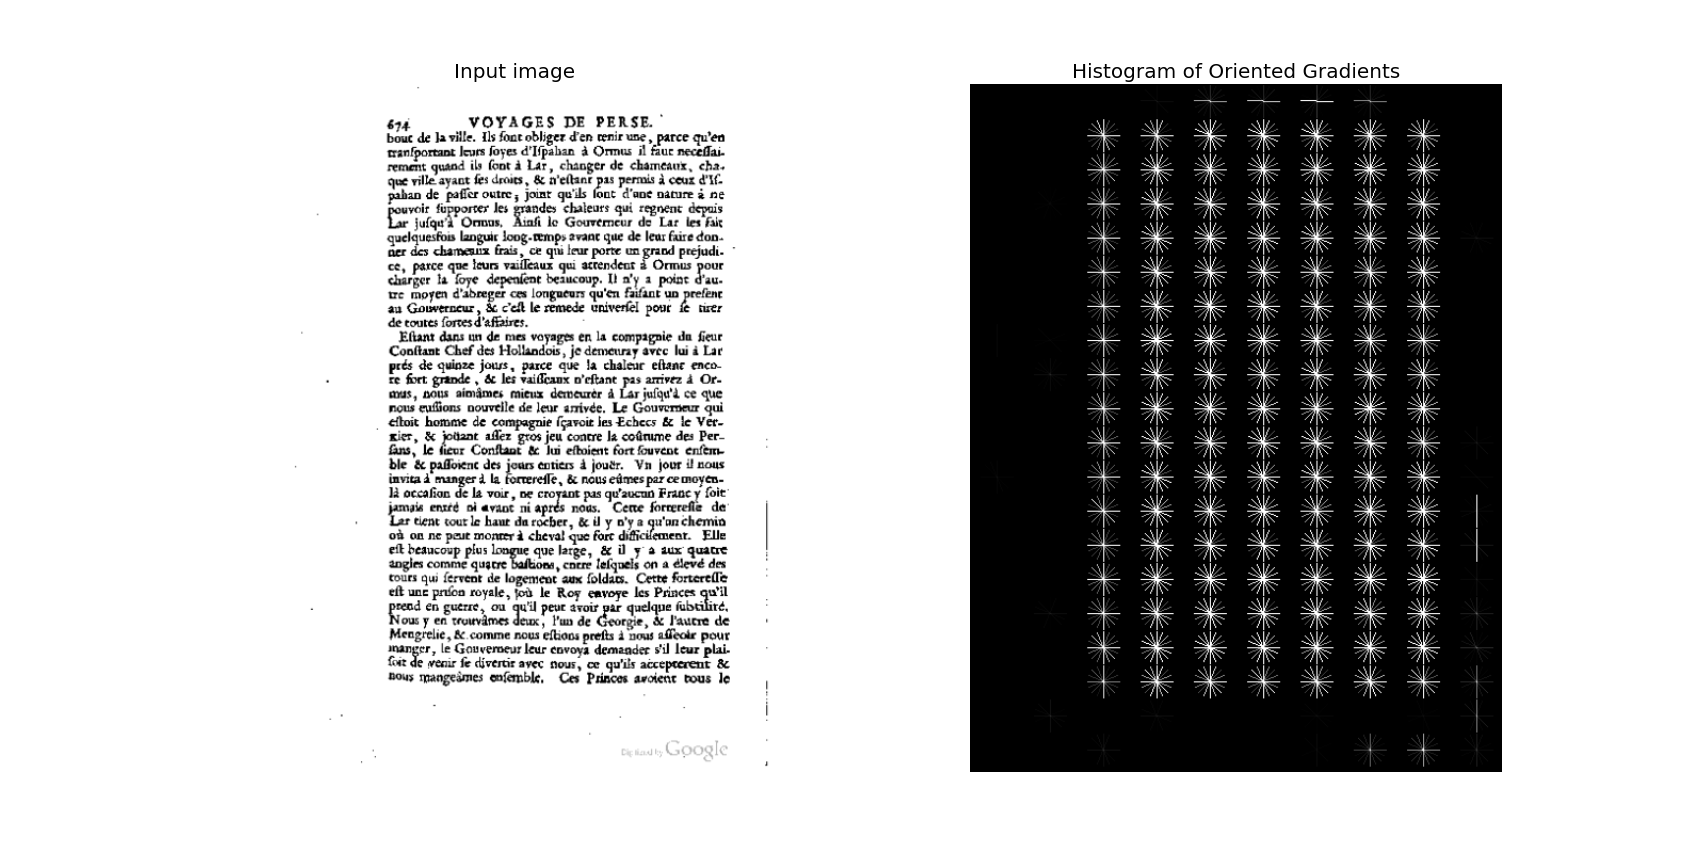
\includegraphics[trim=200px 0px 100px 0px, clip=true, width=.8\paperwidth]{resources/text1}\\
\framebreak
	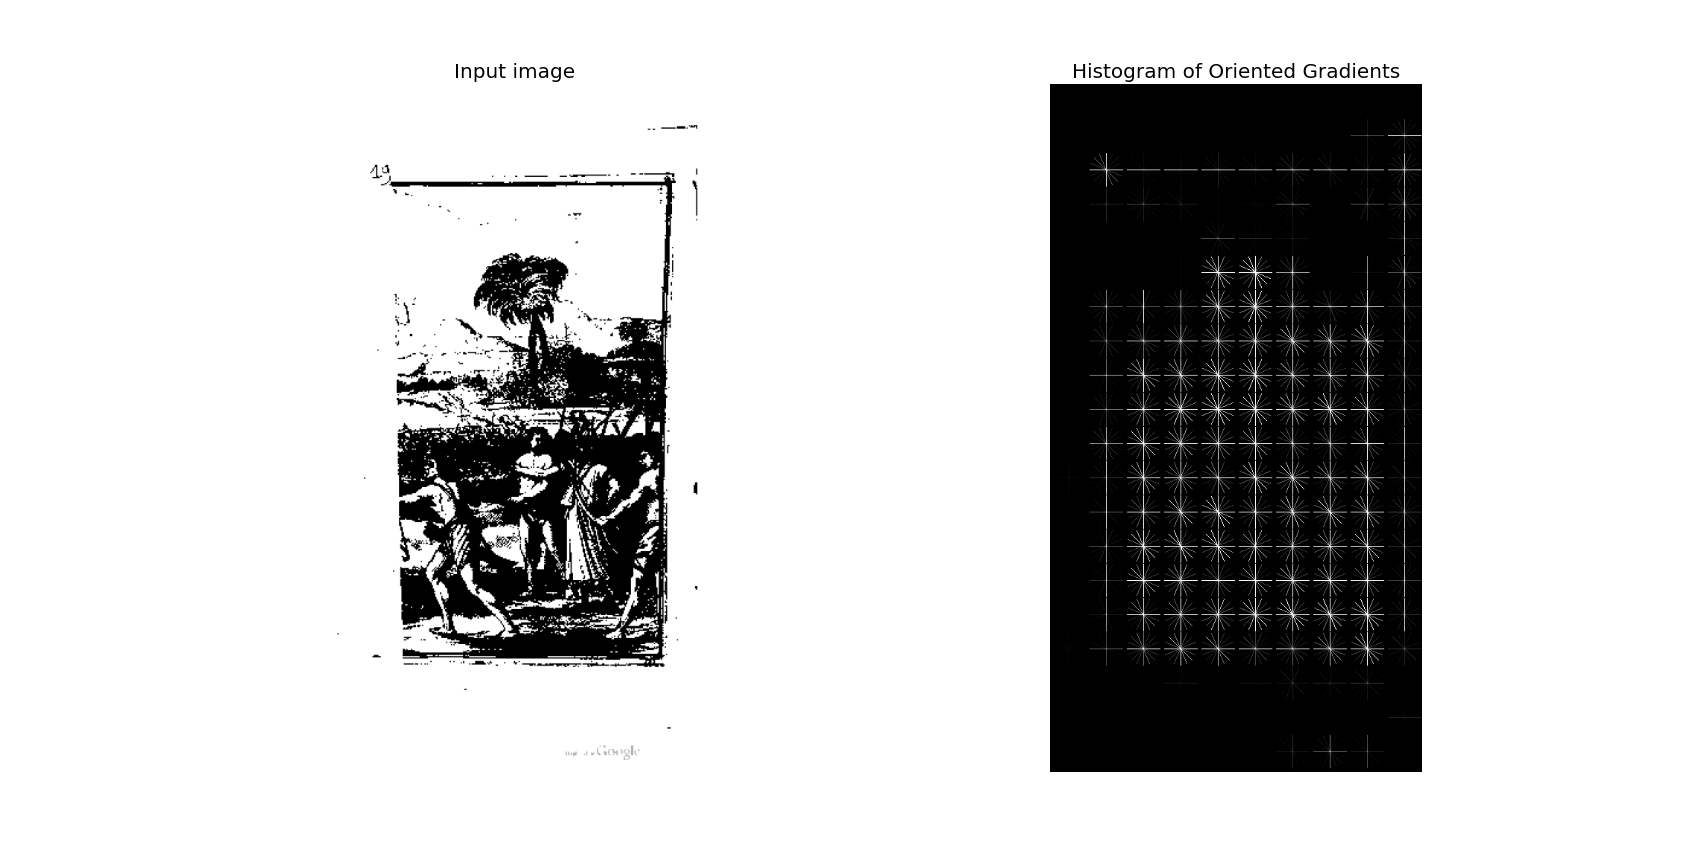
\includegraphics[trim=200px 0px 100px 0px, clip=true, width=.8\paperwidth]{resources/image1}\\
\framebreak
	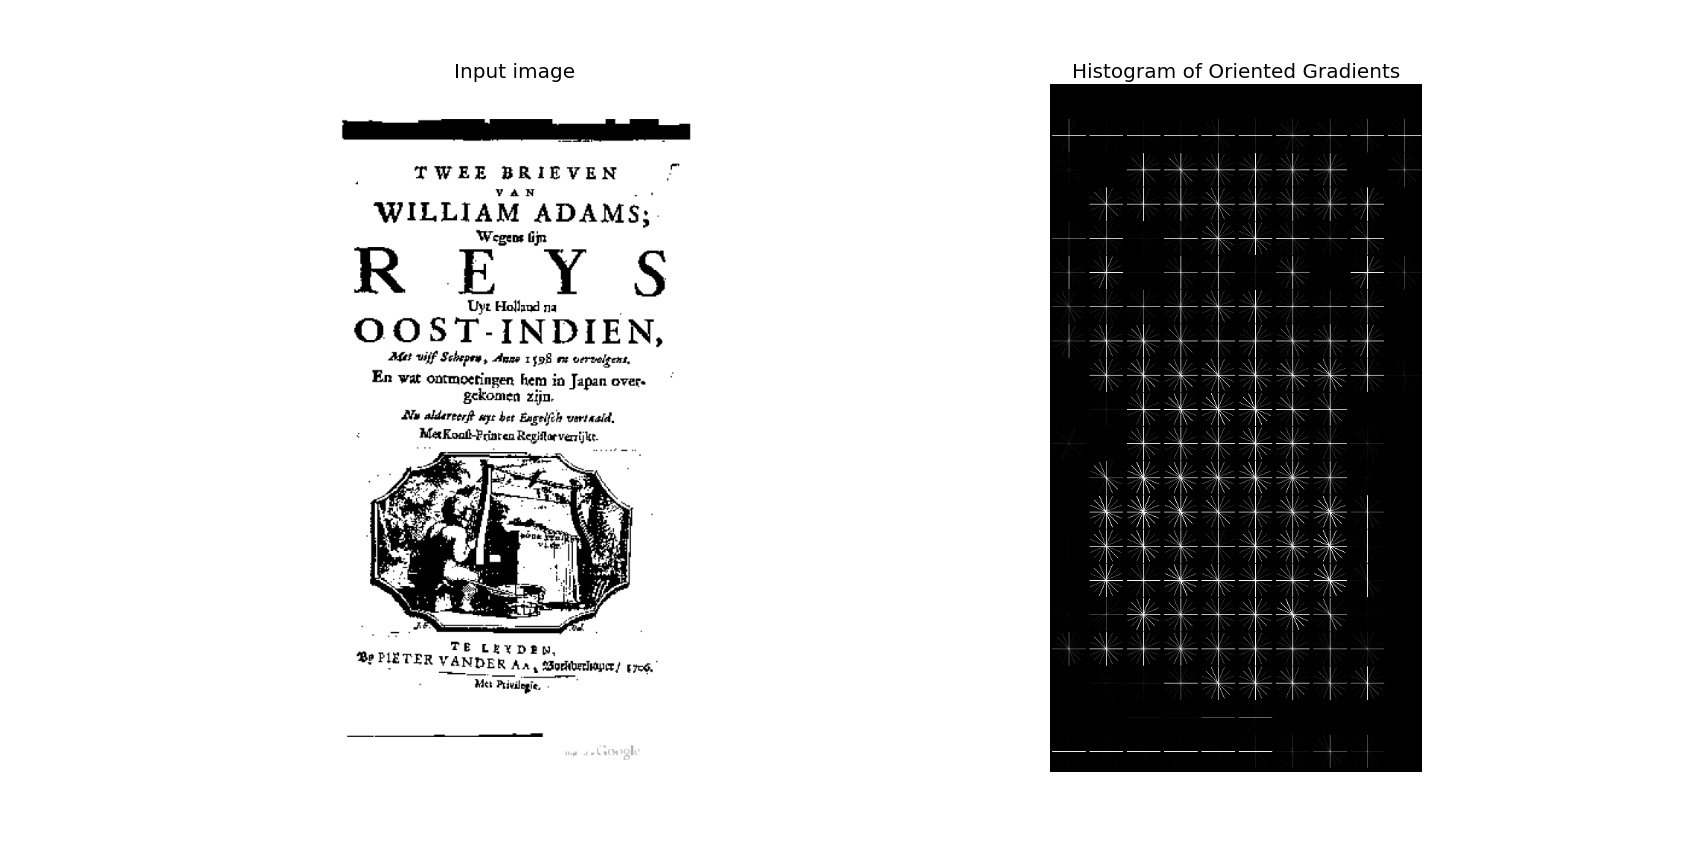
\includegraphics[trim=200px 0px 100px 0px, clip=true, width=.8\paperwidth]{resources/text_and_image1}
\end{frame}

% Explain SVM i.c.w. HOG features for pages
% Moved to introduction
% \slide{Classification using SVM}
% {
% 	\begin{itemize}
% 		\item All pages are annotated with having either ``text'', ``images'' or
% 		``nothing useful'' on it. Images get bounding boxes, which we will later
% 		use.
% 		\item Calculate 5x5 HOG features per page
% 		\item Train a Support Vector Machine (SVM) on these feature vectors and
% 		labels
% 		\item Predict whether a page contains an image based on this SVM
% 	\end{itemize}
% }

\begin{frame}
\frametitle{Test - Validation}
\begin{itemize}
\item Merge the sets of all annoated book pages into one set
\item Split this set into train set ($80\%$) and validation set($20\%$)
\item Use validation set to set parameters ($C$)
\end{itemize}


\end{frame}

\subsection{Results}
\begin{frame}
\frametitle{Results}
\begin{itemize}
\item Run the learned classifier on new books
\item Use F2-score in order to focus on recall (preprocess for annotator)
\end{itemize}
TODO: list results

\end{frame}


\section{Image Localization}

\begin{frame}
\frametitle{Image Locatization}
Second step:
\begin{itemize}
\item find bounding boxes of images on new books
\item classify whether patch is an image or text patch
\item reconstruct images from patches
\end{itemize}
HOG features:
\begin{itemize}
\item 10x20 per page
\item Additionally: concatenate features, 9x19 per page
\end{itemize}
\end{frame}

\subsection{Method}
\begin{frame}
\frametitle{Conditional Random Fields}
\begin{itemize}
\item Regard image as undirected graph (labels $x_i$, patches $y_i$)
\item Decide label for $x_i$ on patch likeliness, neighborhood, and prior
\item Solver: Structural Support Vector Machine (SSVM)
\end{itemize}
$$ E(\mathbf{x}, \mathbf{y}) = h\sum_i x_i - \beta \sum_{\{i, j\}} x_i x_j
- \eta \sum_i x_i y_i $$

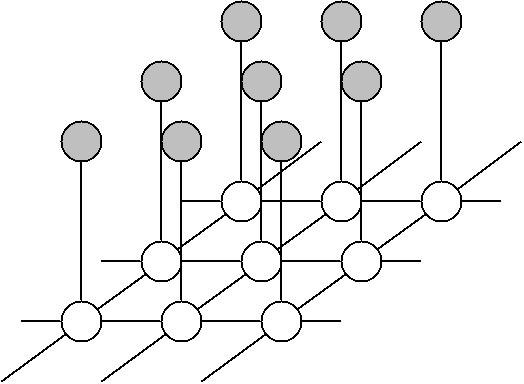
\includegraphics[width=.3\paperwidth]{resources/crf}
\end{frame}

\begin{frame}{CRF and SSVM}

\begin{itemize}
\item To solve the CRF, the energy function must be minimized.
\item For this, two types of SSVMs can be used:
\begin{itemize}
	\item N-slack SSVM
	\item One-slack SSVM
\end{itemize}
\item $\argmin \hat{y} \text{E}(x, y) + \text{loss}(\hat{y}, y) $
\item Where the loss is the \emph{Hamming} loss
\end{itemize}
\end{frame}

\begin{frame}
\frametitle{Preprocess Features Using an SVM}
\begin{itemize}
\item HOG features have 8 values
\item SSVM is harder to solve for more dimensions per feature
\item Use SVM to assign confidence score to each feature
\item Now SSVM has input of 1 dimension per feature
\end{itemize}
\end{frame}

\begin{frame}
\frametitle{Two Stage Training}
Require two stage training to prevent overfitting.
\begin{itemize}
\item Train SVM on $75\%$ of train set, and predict labels on remainder for SSVM
\item Repeat 4 times, with different splits
\item Now $100\%$ of the SSVM features is available
\item Once more: train SVM on $100\%$ of train set to obtain best model
\end{itemize}
\begin{center}
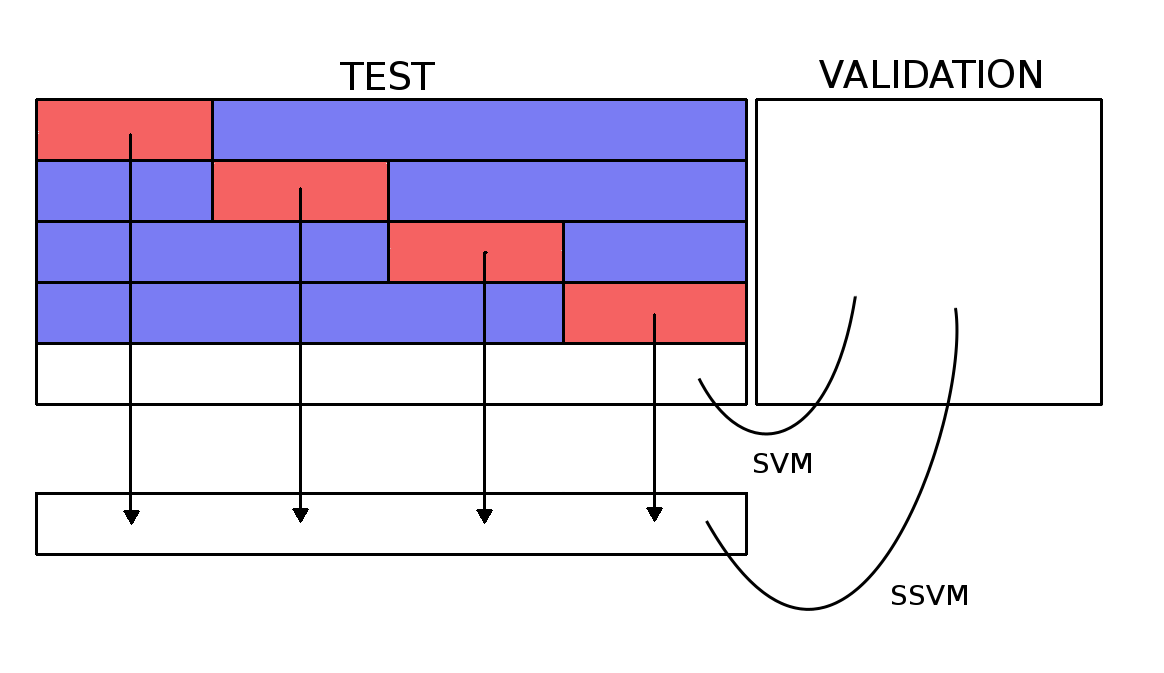
\includegraphics[width=.5\paperwidth]{resources/twostage}
\end{center}
\end{frame}

\subsection{Results}

\begin{frame}
\frametitle{Results}
insert results here
\end{frame}



% Show results for classification
% Show results for different usages of SSVM

\section{Demo}
% Show which images are found (and which are not?) in a live demo

% Improvements: 
% - Different kinds of features
% - 

\section{Discussion \& Conclusion} 

\slide{Discussion \& Conclusion}
{
	Discussion \& Future work:
	\begin{itemize}
		\item Features: We could use different types of features 
		\item Recognize text (OCR)
		\item Different sizes of patches and overlap
	\end{itemize}
	Conclusion:
	\begin{itemize}
		\item An annotator can be used to easily and quickly annotate books with
		lots of text and little images
		\item HOG features can be used to classify pages with images with
		reasonable accuracy
		\item It is not trivial to localize images using only local features.
	\end{itemize}
}
% \begin{frame}[allowframebreaks]
%         \frametitle{References}
%         \bibliographystyle{amsalpha}
%         \bibliography{references.bib}
% \end{frame}

\begin{frame}
Questions?
\end{frame}
\end{document}
